%%%%%%%%%%%%%%%%%%%%%%%%%%%%%%%%%%%%%%%%%%%
%
% From a template maintained at https://github.com/jamesrobertlloyd/cbl-tikz-poster
%
% Code near the top should be fairly standard and not need to be changed
%  - except for the document class
% Code lower down is more likely to be customised
%
%%%%%%%%%%%%%%%%%%%%%%%%%%%%%%%%%%%%%%%%%%%


\documentclass[portrait,a0b,final,a4resizeable]{include/a0poster}

\usepackage{multicol}
\usepackage{color}
\usepackage{morefloats}
\usepackage[pdftex]{graphicx}
\usepackage{rotating}
\usepackage{amsmath, amsthm, amssymb, bm}
\usepackage{array}
\usepackage{booktabs}
\usepackage{multirow}
\usepackage{hyperref}
\usepackage{listings}
\usepackage{xcolor}

\usepackage{include/picins}
\usepackage{tikz}
\usetikzlibrary{shapes.geometric,arrows,chains,matrix,positioning,scopes,calc}
\tikzstyle{mybox} = [draw=white, rectangle]
\definecolor{darkblue}{rgb}{0,0.08,0.45}
\definecolor{blue}{rgb}{0,0,1}

\usepackage{dsfont}
\usepackage{algorithm}
%\usepackage{algorithmic}
\usepackage{algpseudocode}

%%%%%%%%%%%%%%%%%%%%%%%%%%%%%%%%%%%%%%%%%%%
%
% myfig
%
% \myfig - replacement for \figure
% necessary, since in multicol-environment 
% \figure won't work        
%                 
%%%%%%%%%%%%%%%%%%%%%%%%%%%%%%%%%%%%%%%%%%%

\newcommand{\myfig}[3][0]{
\begin{center}
  \vspace{1.5cm}
  \includegraphics[width=#3\hsize,angle=#1]{#2}
  \nobreak\medskip
\end{center}}

%%%%%%%%%%%%%%%%%%%%%%%%%%%%%%%%%%%%%%%%%%%
%
% mycaption                
%
% \mycaption - replacement for \caption
% necessary, since in multicol-environment \figure and
% therefore \caption won't work
%
%%%%%%%%%%%%%%%%%%%%%%%%%%%%%%%%%%%%%%%%%%%

%\newcounter{figure}
\setcounter{figure}{1}
\newcommand{\mycaption}[1]{
  \vspace{0.5cm}
  \begin{quote}
    {{\sc Figure} \arabic{figure}: #1}
  \end{quote}
  \vspace{1cm}
  \stepcounter{figure}
}

%%%%%%%%%%%%%%%%%%%%%%%%%%%%%%%%%%%%%%%%%%%
%
% Some standard colours
%
%%%%%%%%%%%%%%%%%%%%%%%%%%%%%%%%%%%%%%%%%%%

\definecolor{camlightblue}{rgb}{0.601 , 0.8, 1}
\definecolor{camdarkblue}{rgb}{0, 0.203, 0.402}
\definecolor{camred}{rgb}{1, 0.203, 0}
\definecolor{camyellow}{rgb}{1, 0.8, 0}
\definecolor{lightblue}{rgb}{0, 0, 0.80}
\definecolor{white}{rgb}{1, 1, 1}
\definecolor{whiteblue}{rgb}{0.80, 0.80, 1}

%%%%%%%%%%%%%%%%%%%%%%%%%%%%%%%%%%%%%%%%%%%
%
% Some look and feel definitions
%
%%%%%%%%%%%%%%%%%%%%%%%%%%%%%%%%%%%%%%%%%%%

\setlength{\columnsep}{0.03\textwidth}
\setlength{\columnseprule}{0.0018\textwidth}
\setlength{\parindent}{0.0cm}

%%%%%%%%%%%%%%%%%%%%%%%%%%%%%%%%%%%%%%%%%%%
%
% \mysection - replacement for \section*
% 
% Puts a pretty box around some text
% TODO - any other thoughts for what this box should look like
%
%%%%%%%%%%%%%%%%%%%%%%%%%%%%%%%%%%%%%%%%%%%

\tikzstyle{mysection} = [rectangle, 
			draw=none, 
			shade, 
			outer color=camlightblue!0,
			inner color=camlightblue!0,
			text width=0.965\columnwidth,
			text centered,
			rounded corners=20pt,
			minimum height=0.09\columnwidth]

\newcommand{\mysection}[1]
{
\begin{center}
  \begin{tikzpicture}
    \node[mysection] {\sffamily\bfseries\LARGE#1};
  \end{tikzpicture}
\end{center}
}

%%%%%%%%%%%%%%%%%%%%%%%%%%%%%%%%%%%%%%%%%%%
%
% Set the font
%
% TODO - Not sure what a canonical choice is - feel free to modify
%
%%%%%%%%%%%%%%%%%%%%%%%%%%%%%%%%%%%%%%%%%%%

\renewcommand{\familydefault}{cmss}
\sffamily

%%%%%%%%%%%%%%%%%%%%%%%%%%%%%%%%%%%%%%%%%%%%%%%%%%%%
%%%               Background                     %%%
%%%%%%%%%%%%%%%%%%%%%%%%%%%%%%%%%%%%%%%%%%%%%%%%%%%%

\newcommand{\background}[3]{
  %\definecolor{cgradbegin}{#1}
  %\definecolor{cgradend}{#2}
 % \psframe[fillstyle=gradient,gradend=cgradend,
 % gradbegin=cgradbegin,gradmidpoint=#3](0.,0.)(1.\textwidth,-1.\textheight)
}




%%%%%%%%%%%%%%%%%%%%%%%%%%%%%%%%%%%%%%%%%%%%%%%%%%%%
%%%                pcolumn                       %%%
%%%%%%%%%%%%%%%%%%%%%%%%%%%%%%%%%%%%%%%%%%%%%%%%%%%%

\newenvironment{pcolumn}[1]{
  \begin{minipage}{#1\textwidth}
  \begin{center}
}{
  \end{center}
  \end{minipage}
}



%%%%%%%%%%%%%%%%%%%%%%%%%%%%%%%%%%%%%%%%%%%%%%%%%%%%
%%%                pbox                          %%%
%%%%%%%%%%%%%%%%%%%%%%%%%%%%%%%%%%%%%%%%%%%%%%%%%%%%

\definecolor{lcolor}{rgb}{0, 0, 0.80}
\definecolor{gcolor1}{rgb}{1, 1, 1}
\definecolor{gcolor2}{rgb}{.80, .80, 1}

  % \def\fc{fillcolor}
  % \def\getfc #1=#2\par{\def\ffc{#1} \ifx\ffc\fc #2\fi} 
  % \def\getfillcolor #1,#2\par{\getfc #1\par \getfc #2\par}

 %  \newcommand{\psshadowbox}[2]{%[2][magenta]{
%      \fbox{Input arg: #1}
%      \fbox{#1} 
%      \fbox {\getfillcolor #1\par}
%      \def\col{\getfillcolor #1\par}
 
%      \let\coll=\col
%       \coll
 %     \colorbox{\col}{#2}
%       \mbox
   %   \coloredshadowbox{black}{\coll}{#2}
%   }

\newcommand{\pbox}[4]{
%\psshadowbox[#3]{
%\fbox{
\mbox{
\begin{minipage}[t][#2][t]{#1}
#4
\end{minipage}
}%}
}

%%%%%%%%%%%%%%%%%%%%%%%%%%%%%%%%%%%%%%%%%%%
%
% Poster environment
%
% Centres everything and can be used to define the width of the content
%
%%%%%%%%%%%%%%%%%%%%%%%%%%%%%%%%%%%%%%%%%%%

\newenvironment{poster}{
  \begin{center}
  \begin{minipage}[c]{\textwidth}
}{
  \end{minipage}
  \end{center}
}

\def\newarrow{\mbox{\begin{tikzpicture}
             \useasboundingbox{(-3pt,-4.5pt) rectangle (19pt,1pt)};
             \draw[->] (0,-0.07)--(17pt,-0.07);\end{tikzpicture}}}



%\ProvidesPackage{preamble}

\usepackage{url}
\usepackage{array}
\usepackage{amsmath,amssymb,amsfonts,textcomp}
\usepackage{booktabs}
\usepackage{relsize}
\usepackage{nicefrac}
\usepackage{graphicx}
\usepackage{rotating}
\usepackage{nth}
\usepackage{acronym}
\usepackage{bm}

\newcommand{\binarysum}{\sum_{\bf{x} \in \{0,1\}^D}}
\newcommand{\expect}{\mathbb{E}}
\newcommand{\expectargs}[2]{\mathbb{E}_{#1} \left[ {#2} \right]}
\newcommand{\var}{\mathbb{V}}
\newcommand{\varianceargs}[2]{\mathbb{V}_{#1} \left[ {#2} \right]}
\newcommand{\variance}{\mathbb{V}}
\newcommand{\cov}{\operatorname{cov}}
\newcommand{\Cov}{\operatorname{Cov}}
\newcommand{\covarianceargs}[2]{\Cov_{#1} \left[ {#2} \right]}
\newcommand{\colvec}[2]{\left[ \begin{array}{c} {#1} \\ {#2} \end{array} \right]}
\newcommand{\tbtmat}[4]{\left[ \begin{array}{cc} {#1} & {#2} \\ {#3} & {#4} \end{array} \right]}

%\newcommand{\covskinny}[2]{\var\!\left(#1\middle\vert#2\right)} 

\newcommand{\acro}[1]{\textsc{#1}}
%\newcommand{\vect}[1]{\boldsymbol{#1}}
\newcommand{\vect}[1]{{\bf{#1}}}
\newcommand{\mat}[1]{\mathbf{#1}}
\newcommand{\pderiv}[2]{\frac{\partial #1}{\partial #2}}
\newcommand{\npderiv}[2]{\nicefrac{\partial #1}{\partial #2}}

\newcommand{\pha}{^{\phantom{:}}}

\newcommand{\argmin}{\operatornamewithlimits{argmin}}
\newcommand{\argmax}{\operatornamewithlimits{argmax}}

% The following designed for probabilities with long arguments

\newcommand{\Prob}[2]{P\!\left(\,#1\;\middle\vert\;#2\,\right)}
\newcommand{\ProbF}[3]{P\!\left(\,#1\!=\!#2\;\middle\vert\;#3\,\right)}
\newcommand{\p}[2]{p\!\left(#1\middle\vert#2\right)}
\newcommand{\po}[1]{p\!\left(#1\right)}
\newcommand{\pF}[3]{p\!\left(\,#1\!=\!#2\;\middle\vert\;#3\,\right)} 
\newcommand{\mean}[2]{{m}\!\left(#1\middle\vert#2\right)}
%\newcommand{\novmean}[2]{{m}\!\left(#1\middle\vert#2\right)}
%\newcommand{\novcov}[2]{\var\!\left(#1\middle\vert#2\right)}
%\newcommand{\cov}[2]{\var\!\left(#1\middle\vert#2\right)} 
%\newcommand{\pskinny}[2]{p\!\left(#1\;\middle\vert\;#2\right)}
%\newcommand{\meanskinny}[2]{{m}\!\left(#1\middle\vert#2\right)}
%\newcommand{\covskinny}[2]{\var\!\left(#1\middle\vert#2\right)} 

\newcommand{\vI}{\mat{I}}
\newcommand{\vX}{\mat{X}}
\newcommand{\vY}{\mat{Y}}
\newcommand{\vZ}{\mat{Z}}
\newcommand{\vK}{\mat{K}}
\newcommand{\vs}{\vect{s}}
\newcommand{\va}{\vect{a}}
\newcommand{\vA}{\vect{A}}
\newcommand{\vb}{\vect{b}}
\newcommand{\vB}{\mat{B}}
\newcommand{\vR}{\mat{R}}
\newcommand{\vS}{\mat{S}}
\newcommand{\vu}{\vect{u}}
\newcommand{\vk}{\vect{k}}
\newcommand{\vc}{\vect{c}}
\newcommand{\vC}{\mat{C}}
\newcommand{\vw}{\vect{w}}
\newcommand{\vx}{\vect{x}}
\newcommand{\vy}{\vect{y}}
\newcommand{\vz}{\vect{z}}
\newcommand{\vmu}{\vect{\mu}}
\newcommand{\vpi}{\vect{\pi}}
\newcommand{\vphi}{\vect{\phi}}
\newcommand{\vSigma}{\mat{\Sigma}}
\newcommand{\vtheta}{\vect{\theta}}
\newcommand{\vl}{\vect{l}}
\newcommand{\vq}{\vect{q}}
\newcommand{\vf}{\vect{f}}
\newcommand{\vg}{\vect{g}}
\newcommand{\vell}{\vect{\ell}}
\newcommand{\ve}{\vect{\epsilon}}
\newcommand{\vzero}{\vect{0}}
\newcommand{\vone}{\vect{1}}

\newcommand{\He}{\mathcal{H}}
\newcommand{\normx}[2]{\left\|#1\right\|_{#2}}
\newcommand{\Hnorm}[1]{\normx{#1}{\He}}
\newcommand{\mmd}{{\rm MMD}}


\newcommand{\mf}{\bar{\vf}}

\newcommand{\st}{_\star}

\newcommand{\inv}{^{{\mathsmaller{-1}}}}
\newcommand{\tohalf}{^{{\mathsmaller{\nicefrac{1}{2}}}}}

\newcommand{\N}[3]{\mathcal{N}\!\left(#1|#2,#3\right)}
\newcommand{\bN}[3]{\mathcal{N}\big(#1|#2,#3\big)}
\newcommand{\boldN}[3]{\text{\textbf{\mathcal{N}}}\big(#1;#2,#3\big)}
\newcommand{\ones}[1]{\mat{1}_{#1}}
\newcommand{\eye}[1]{\mat{E}_{#1}}
\newcommand{\tra}{^\ensuremath{\mathsf{T}}}
\newcommand{\trace}{\operatorname{tr}}
\newcommand{\deq}{:=}
\newcommand{\degree}{^\circ}

\DeclareMathOperator{\chol}{chol}
\DeclareMathOperator{\diag}{diag}

\newcommand{\gp}{{\acro{gp}}}
\newcommand{\bmc}{{\acro{bmc}}}
\newcommand{\bq}{{\acro{bq}}}
\newcommand{\sbq}{{\acro{sbq}}}

\newenvironment{narrow}[2]{%
  \begin{list}{}{%
  \setlength{\topsep}{0pt}%
  \setlength{\leftmargin}{#1}%
  \setlength{\rightmargin}{#2}%
  \setlength{\listparindent}{\parindent}%
  \setlength{\itemindent}{\parindent}%
  \setlength{\parsep}{\parskip}}%
\item[]}{\end{list}}

\newtheorem{prop}{Proposition}
\newtheorem{cor}{Corollary}
\newtheorem{lem}{Lemma}


\def\ie{i.e.\ }
\def\eg{e.g.\ }
\def\iid{i.i.d.\ }
\def\simiid{\sim_{\mbox{\tiny iid}}}
\def\eqdist{\stackrel{\mbox{\tiny d}}{=}}

\def\Reals{\mathbb{R}}

\def\Uniform{\mbox{\rm Uniform}}
\def\Bernoulli{\mbox{\rm Bernoulli}}
\def\GP{\mathcal{GP}}

\def\inputVar{x}
\def\InputVar{X}
\def\InputSpace{\mathcal{X}}
\def\outputVar{y}
\def\OutputSpace{\mathcal{Y}}
\def\function{f}
\def\kernel{k}
\def\KernelMatrix{K}
\def\SumKernel{\sum}
\def\ProductKernel{\prod}
\def\expression{e}

\def\SE{\acro{SE}}
\def\Per{\acro{Per}}
\def\RQ{\acro{RQ}}
\def\Lin{\acro{Lin}}

\def\subexpr{{\cal S}}
\def\baseker{{\cal B}}
\def\numWinners{k}

\newcommand{\kSE}{{\acro{SE}}}
\newcommand{\kC}{{\acro{C}}}
\newcommand{\kPer}{{\acro{Per}}}
\newcommand{\kLin}{{\acro{Lin}}}
\newcommand{\kWN}{{\acro{WN}}}
\newcommand{\kCP}{{\acro{CP}}}
\newcommand{\kCW}{{\acro{CW}}}
\newcommand{\kRQ}{{\acro{RQ}}}

%\newcommand{\vv}{\mathbf{v}}

\definecolor{myfavblue}{rgb}{0.1176, 0.392, 1.0}

% Math typesetting.
\newcommand{\vx}{\mathbf{x}}
\newcommand{\vX}{\mathbf{X}}
\newcommand{\vw}{\mathbf{w}}
\newcommand{\vv}{\mathbf{v}}
\newcommand{\vr}{\mathbf{r}}
\newcommand{\vg}{\mathbf{g}}
\newcommand{\vI}{\mathbf{I}}
\newcommand{\vzero}{\bf{0}}
\newcommand{\ones}[1]{\mat{1}_{#1}}
\newcommand{\eye}[1]{\mat{E}_{#1}}
\newcommand{\tra}{^{\mathsf{T}}}
\newcommand{\vect}[1]{{\bf{#1}}}
\newcommand{\mat}[1]{\mathbf{#1}}
\newcommand{\pderiv}[2]{\frac{\partial #1}{\partial #2}}
\newcommand{\npderiv}[2]{\nicefrac{\partial #1}{\partial #2}}
\newcommand{\argmin}{\operatornamewithlimits{argmin}}
\newcommand{\argmax}{\operatornamewithlimits{argmax}}
\newcommand{\expect}{\mathbb{E}}
\newcommand{\expectargs}[2]{\mathbb{E}_{#1} \left[ {#2} \right]}
\newcommand{\var}{\mathbb{V}}
\newcommand{\varL}{\mathcal{L}}
\def\iid{i.i.d.\ }
\def\simiid{\overset{\mbox{\tiny iid}}{\sim}}
\newcommand{\defeq}{\mathrel{:\mkern-0.25mu=}}
\newcommand{\Normal}{\mathcal{N}}
\newcommand{\Nt}[3]{\mathcal{N}\!\left(#1 \middle| #2,#3\right)}
\newcommand{\N}[2]{\mathcal{N}\!\left(#1,#2\right)}
\DeclareMathOperator{\KLop}{KL}
\newcommand{\KL}[2]{\KLop \left(#1 \middle \| #2 \right)}

% Symbol definitions.
\newcommand{\distinit}{q_0(\params, \vv)}
\newcommand{\data}{\vx}

%% \newcommand{\params}{\vx}
\newcommand{\params}{\mathbf{\theta}}
\newcommand{\trans}{T}
\newcommand{\paramsrv}{\vX}  % Random variable.
\newcommand{\numsteps}{T}
\newcommand{\decay}{\gamma}
\newcommand{\decays}{{\boldsymbol{\decay}}}
\newcommand{\stepsize}{\alpha}
\newcommand{\stepsizes}{{\boldsymbol{\stepsize}}}
\newcommand{\gradparams}{\nabla L(\params_t, t)}
\DeclareMathOperator{\SGD}{SGD}
\newcommand{\entropy}{S}
\newcommand{\pun}{{\tilde p}}
\newcommand{\jointdist}{p(\params , \data)}
\newcommand{\posterior}{p(\params | \data)}
\newcommand{\subjointdist}[2]{p_{#1}(\params_{#2} , \data)}
\newcommand{\subjointdistminibatch}[1]{\tilde{p}(\params_{#1} , \data)}
\newcommand{\reals}{\mathbb{R}}
\newcommand{\bigo}[1]{\mathcal{O}\left(#1\right)}
%\newcommand{\trace}[1]{\text{Tr}\left[#1\right]}
\newcommand{\loss}{L(\params)}


\definecolor{Blue}{rgb}{0.0,0.0,1.0}
\definecolor{Black}{rgb}{0.0,0.0,0.0}
\definecolor{Green}{rgb}{0.0,0.8,0.0}
\definecolor{Purple}{rgb}{1.0,0.0,1.0}
\lstloadlanguages{Python}%
\lstset{language=Python,
        frame=none,
        basicstyle=\small\ttfamily\bfseries,
        keywordstyle=[1]\color{Blue},
        keywordstyle=[2]\color{Purple},
        commentstyle=\usefont{T1}{pcr}{m}{sl}\color{Green},
        keepspaces=true,
        }
%\lstset{language=Python}
\lstset{
 morekeywords={sum, exp, max, log, full, defgrad, shape}
}


\begin{document}
\begin{poster} 


%%% Header
\begin{center}
\begin{pcolumn}{0.99}

\newcommand{\logowidth}{0.13\textwidth}

\pbox{0.99\textwidth}{}{linewidth=2mm,framearc=0.3,linecolor=camdarkblue,fillstyle=gradient,gradangle=0,gradbegin=white,gradend=white,gradmidpoint=1.0,framesep=1em}{
%
%%% Cambridge Logo
\begin{minipage}[c]{\logowidth}
  %\begin{center}
    
\includegraphics[width=16cm]{badges/hips-logo.png}
  %\end{center}
\end{minipage}
%
%%% Title
\begin{minipage}[c][9cm][c]{0.7\textwidth}
  \begin{center}
    {\sffamily \VeryHuge \textbf{Early Stopping is Nonparametric \\Variational Inference}}\\[10mm]
    {\huge\sffamily \Huge David Duvenaud*, Dougal Maclaurin*, Ryan Adams\\[7.5mm]}
  \end{center}
\end{minipage}
%
%
% Harvard logo
\begin{minipage}[c]{\logowidth}
  \begin{flushright}
    
\includegraphics[width=9cm,trim=2em 0em 2em 2em, clip]{badges/harvard}
  \end{flushright}
\end{minipage}
%
}
\end{pcolumn}
\end{center}

\vspace*{1.5cm}

\Large


%%%%%%%%%%%%%%%%%%%%%%%%%%%%%%%%%%%%%%%%%%%%%%%%%%%%%%%%%%%%%%%%%%%%%%
%%% Beginning of Document
%%%%%%%%%%%%%%%%%%%%%%%%%%%%%%%%%%%%%%%%%%%%%%%%%%%%%%%%%%%%%%%%%%%%%%

\begin{multicols}{2}

\mysection{Why does early stopping help?}

%\vspace{0.5in}

%\begin{minipage}[c]{0.17\columnwidth}

\begin{centering}
\begin{tabular}{rcl}
Regularization & $=$ & MAP inference \\
Limiting model capacity & $=$ &Bayesian Occam's razor \\
Cross-validation & $=$ &Estimating marginal likelihood \\
Dropout        & $=$ &Integrating out spike-and-slab \\
Ensembling & $=$ &Bayes model averaging? \\
Early stopping & $=$ & ??
\end{tabular}
\end{centering}

\vspace{0.5in}
\mysection{Gradient descent with random starts is a sampler}

What is the implicit distribution of parameters after optimizing for $t$ steps?
\vspace{0.5in}
\newcommand{\dist}[1]{\includegraphics[width=0.33\columnwidth]{../experiments/2015_03_02_funnel/6-nicer/figures/dists_#1.pdf}}%
\setlength{\tabcolsep}{2pt}
\begin{tabular}{ccc}
Initial distribution & After 150 steps & After 300 steps \\
\dist{0} &
\dist{3} &
\dist{6}
\end{tabular}

Distributions (blue) implicitly defined by gradient descent on an objective (black).
\vspace{0.5in}
\begin{itemize} 
\item Starts as a bad approximation (prior dist)
\item Ends as a bad approximation (point mass)
\item Ensembling $=$ taking multiple samples from dist
\item Early stopping $=$ choosing best intermediate dist
\end{itemize}

\vspace{0.5in}
\mysection{Cross validation vs. marginal likelihood}
\vspace{-0.5in}

\begin{itemize} 
\item What if we could evaluate marginal likelihood of implicit distribution?
\item Could choose all hypers to maximize marginal likelihood
\item No need for cross-validation?
\end{itemize}

\vspace{0.5in}
\mysection{Contribution: Variational Lower Bound}
\vspace{-1in}

\begin{align*}
\log p(\data) \geq - \underbrace{\expectargs{q(\params)}{ -\log \jointdist }}_{\textnormal{\normalsize Energy $E[q]$}}
 \quad \underbrace{- \expectargs{q(\params)}{\log q(\params)}}_{\textnormal{\normalsize Entropy $S[q]$}}
%& := \varL[q] \label{eq:varbound}
\end{align*}
Energy estimated from optimized objective function (training loss is NLL):
\begin{align*}
\expectargs{q(\params)}{-\log \jointdist} & \approx - \log p(\hat\theta_T, \vx) %\subjointdist{}{T}
\end{align*}
Entropy estimated by tracking change at each iteration:
\begin{align*}
- \expectargs{q(\params)}{\log q(\params)} & \approx S[q_0] + \sum_{t=0}^{T-1} \log \left| J(\hat\params_t) \right|
\label{eq:entropy-bound}
\end{align*}
Using a single sample!


\vspace{0.5in}
\mysection{Estimating change in entropy}
\vspace{-0.5in}
\begin{itemize} 
\item Inuitively: High curvature makes entropy decrease quickly
\item Can measure local curvature with Hessian
\item Approximation good for small step-sizes
\end{itemize}

Volume change given by Jacobian of optimizer's operator:
\begin{align*}
S[q_{t+1}] - S[q_t] = \expect_{q_t(\params_t)} \left[ \log \Big| J(\params_t) \Big| \right]
\end{align*}

Gradient descent update rule:
\begin{align*}
\params_{t+1} &=
  \params_t - \stepsize \nabla \loss,
\end{align*}

Has Jacobian:
\begin{align*}
J(\params_t) = I - \stepsize \nabla \nabla L(\theta_t)
\end{align*}

Entropy change estimated at a single sample:
\begin{align*}
S[q_{t+1}] - S[q_t] \approx \log \left| I - \stepsize \nabla \nabla L(\theta_t) \right|
\end{align*}

\newpage %%%%%%%%%%%%%%%%%%%%%%%%%%%%%%%%%%%%%%%%%%%%%%%%%%%%%%%%%%%%%%%%%%%%%%%%%%%%%%%%%%%%%%%%%%%%%%%


\vspace{0.5in}
\mysection{SGD with entropy estimate}
\begin{algorithmic}[1]
%\scriptsize%
\State {\bfseries input:}
	Weight init scale $\sigma_0$, step size $\stepsize$,
	negative log-likelihood $L(\params, t)$
	\State {\bfseries initialize} $\params_0 \sim \N{0}{\sigma_0 \vI_D}$
	\State {\color{myfavblue}{{\bfseries initialize} $\entropy_{0} = \frac{D}{2} (1 + \log 2 \pi) + D \log\sigma_0$}}
	\For{$t=1$ {\bfseries to} $T$}
		\State {\color{myfavblue}$\entropy_{t} = \entropy_{t-1} + \log \left| \vI - \stepsize \nabla \nabla L(\theta_t, t) \right|$} %\Comment{Update entropy} 
		\State $\params_{t} = \params_{t-1} - \stepsize \gradparams$ % \Comment{Update parameters}	
   \EndFor
   \State \textbf{output} sample $\params_T$, \color{myfavblue}{entropy estimate $\entropy_T$}
\end{algorithmic}





\vspace{0.5in}
\mysection{Computational Complexity}

\begin{itemize}
\item Approximate bound: $\log p(\data) \gtrsim -L(\theta_T) + S_T$
\item Determinant is $\mathcal{O}(D^3)$
\item $\mathcal{O}(D)$ Taylor approximation using Hessian-vector products
\item Scales linearly in parameters and dataset size
\end{itemize}


\vspace{0.5in}
\mysection{Example: Choosing when to stop}

\begin{tabular}{ccc}
\begin{minipage}[c]{0.35\columnwidth}
\begin{itemize} 
\item Neural network on the Boston housing dataset.
\item SGD marginal likelihood estimate gives stopping criterion without a validation set
\end{itemize}
\end{minipage} & \quad &
\begin{minipage}[c]{0.55\columnwidth}
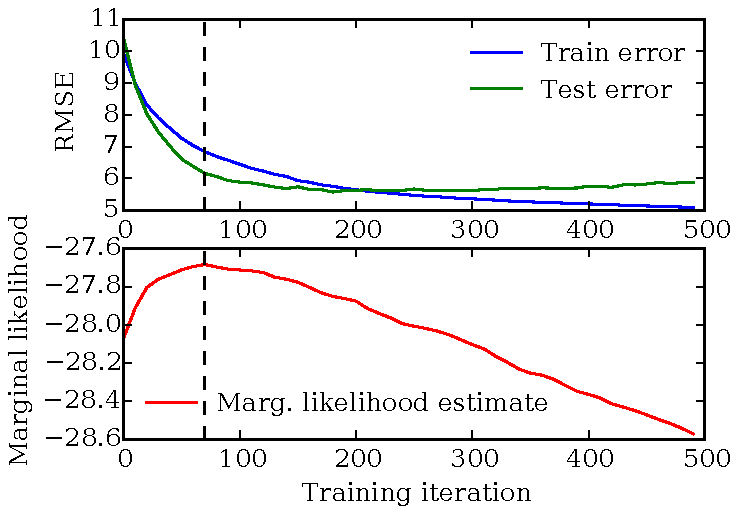
\includegraphics[width=\columnwidth]{../experiments/2015_03_01_housing/2/marglik.pdf}
\end{minipage}
\end{tabular}

\vspace{0.5in}
\mysection{Example: Choosing number of hidden units}

\begin{tabular}{ccc}
\begin{minipage}[c]{0.35\columnwidth}
\begin{itemize} 
\item Neural net on 50000 MNIST digits
\item Largest model has 2 million params
\item Gives reasonable estimates, but cross-validation still better
\item Entropy bound over-penalizes after long training
\end{itemize}
\end{minipage} & &
\begin{minipage}[c]{0.55\columnwidth}
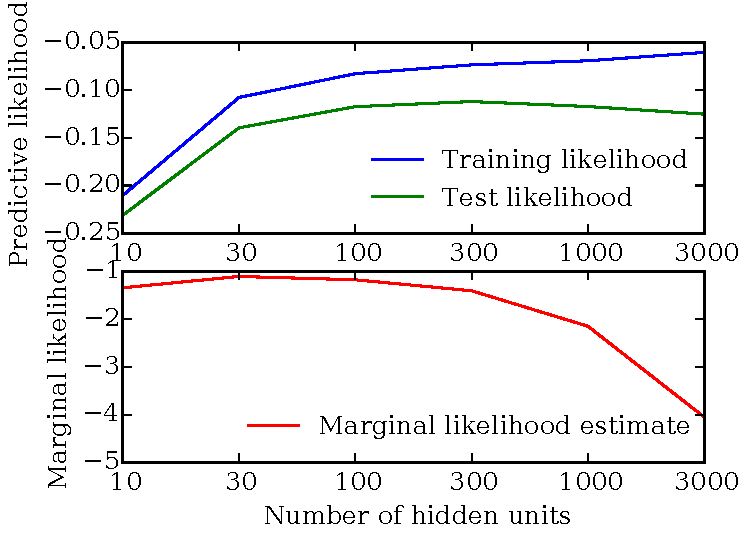
\includegraphics[width=\columnwidth]{../experiments/2015_03_03_vary_width/7_hidden_units_higher_learnrate/vary_widths.pdf}
\end{minipage}
\end{tabular}


\vspace{0.5in}
\mysection{Main Takeaways}
\begin{itemize}
\item Optimization with random restarts implies nonparametric intermediate dists
\item Early stopping chooses among these distributions
\item Ensembling samples from them
\item Can scalably estimate lower bound on model evidence during optimization
\item Bound can be used for Langevin-dynamics recognition networks!
\item All code at {\color{Blue}{\href{http://github.com/HIPS/maxwells-daemon/}{\texttt{github.com/HIPS/maxwells-daemon}}}}
\end{itemize}


\end{multicols}
\end{poster}

\end{document}

